\documentclass[12pt]{report}
\usepackage{pacchetto}
\title{APPUNTI TEORIA DELL'INFORMAZIONE}
\author{Andrea Cosentino}

\def\blankpage{%
    \clearpage%
    \thispagestyle{empty}%
    \addtocounter{page}{-1}%
    \null%
    \clearpage}
\begin{document}
    \maketitle
    \tableofcontents

    \newpage
    \clearpage%
    \thispagestyle{empty}%
    \addtocounter{page}{-1}%
    \null%

    \begin{flushright}
        \begin{tabular}{r}
            \textit{Nel cielo non c'è nulla,}
            \\
            \textit{
                perché le cose importanti stanno per terra.}
            \\
            \begin{footnotesize}
                - Uno studente di teoria dell'informazione.
            \end{footnotesize}
        \end{tabular}
    \end{flushright}

    \clearpage
    \pagecolor{color}
    \blankpage
    \nopagecolor
    \chapter{Lezione I}
    \label{cap:Lezione I}
    \section{Introduzione}

    Durante il corso del '900 diverse figure hanno contribuito allo sviluppo delle fondamenta della disciplina. Tra queste ricordiamo coloro che vengono considerati i padri della disciplina:
    \begin{itemize}
        \item Claude Shannon(USA): primo in assoluto. Fa una definizione in media
        \item Kolmogorov(URSS): arriva dopo Shannon ma fa una definizione puntuale. Espande il lavoro di Shannon.
        \item Chaitin e Solomonoff: arrivano allo stesso tempo di Kolmogorov ma non vengonono considerati perché Kolmogorov era, ed è, più importante a livello accademico.
    \end{itemize}
    \vspace{10px}
    Durante questo corso ci proponiamo di riuscire a spedire dei dati da una sorgente a una destinazione
    attraverso un canale che può essere affetto da rumore.
    \\ \\
    Obiettivi del corso:
    \begin{itemize}
        \item{Sfruttare al massimo il canale}
        \item{Gestire i bit persi nella trasmissione}
    \end{itemize}
    \vspace{10px}
    \newpage
    \section{Una visione d'insieme}

    \begin{tikzpicture}[
        roundnode/.style={circle, draw=green!60, fill=green!5, very thick, minimum size=7mm},
        squarednode/.style={rectangle, draw=red!60, fill=red!5, very thick, minimum width=30mm, minimum height= 10mm},
        curly/.style={decorate,decoration={snake,post length=0.7mm}}
    ]
%Nodes
        \node[squarednode](sorgente){SORGENTE};
        \node[squarednode](rumore)[right=of sorgente] {RUMORE};
        \node[squarednode](ricevente)[right=of rumore]{RICEVENTE};

        \node[squarednode](codifica)[below=of sorgente]{CODIFICA};
        \node[squarednode](canale)[right=of codifica]{CANALE};
        \node[squarednode](decodifica)[right=of canale]{DECODIFICA};

        \draw[->] (sorgente.south) -- (codifica.north);
        \draw[->] (codifica.east) -- (canale.west);
        \draw[->] (canale.east) -- (decodifica.west);
        \draw[->] (decodifica.north) -- (ricevente.south);
        \draw[->,curly] (rumore.south) -- (canale.north);

    \end{tikzpicture}

    \noindent
    Shannon modella l'ambiente come composto da 3 attori:
    \begin{itemize}
        \item \textbf{Sorgente}: La sorgente genera il messaggio, lo codifica e lo spedisce sul canale.
        \item \textbf{Canale}: Il canale è il tramite tra la sorgente e la destinazione. E' il "posto" in cui passa l'informazione. E' affetto da \textbf{rumore}.
        \item \textbf{Ricevente}: Riceve il messaggio codificato. E' suo compito riuscirlo a decodificare.
    \end{itemize}
    \vspace{10px}
    Vogliamo codificare messaggi sorgente \\ \\ (A) Massimizzando informazioni trasmesse A OGNI utilizzo del canale (problema di \textbf{Source coding}) \\ \\ (B) Minimizzando, simultaneamente al primo punto, il numero di errori di trasmissione dovuti al rumore (problema di \textbf{Channel coding}).

    \vspace{5px}
    \noindent
    Shannon cerca di risolvere questo problema usando l'approccio divide et impera. Non è detto che questo approccio sia quello giusto. Infatti, non c'è garanzia che la soluzione ottimale dei due sottoproblemi sia tale che , se messe assieme, diano la soluzione ottimale per il problema. Questo perché potremmo non sfruttare possibili vantaggi di un problema sull'altro. Vale il seguente teorema:
    \vspace{5px}
    \begin{tcolorbox}
        \textbf{\textcolor{red}{TEOREMA} di codifica sorgente e canale}
        \vspace{5px}
        \begin{center}
            L'unione delle soluzioni di source coding e channel coding (quindi dei due sottoproblemi risolti come indipendenti) dà la soluzione ottima.
        \end{center}
    \end{tcolorbox}

    \vspace{10px}

    \newpage
    \noindent Come si risolve il problema del source coding? Enunciamo, in maniera non formale per adesso, il primo teorema di Shannon.
    \vspace{5px}
    \begin{tcolorbox}
        \textbf{\textcolor{red}{TEOREMA} I teorema di Shannon}
        \vspace{5px}
        \begin{center}
            Si può comprimere, tramite un codice, un messaggio con perdite di informazioni piccole
        \end{center}
    \end{tcolorbox}
    \vspace{5px}
    \noindent Questo è dovuto al fatto che l'informazione non è uniformemente distribuita. Ci sono parti della codifica inutile. Per esempio, se codifichiamoun cielo tutto azzurro, non abbiamo bisogno di dire che ogni pixel è di colore azzurro, ma ci basta dire che una porzione di una foto è tutta azzurra.
    \\
    La codidfica, cioè la rimozione della ridondanza, va ad amplificare il problema del rumore. Ogni bit perso è significativo. Per risolvere il problema di channel coding useremo il secondo teorema di Shannon. Anche questo lo riportiamo, per ora, in modo informale.

    \vspace{5px}
    \begin{tcolorbox}
        \textbf{\textcolor{red}{TEOREMA} II teorema di Shannon}
        \vspace{5px}
        \begin{center}
            Possiamo trasmettere con possibilità di errore piccola a piacere. Uitlizziamo una ridondanza, controllata in base alla distorsione del canale.
        \end{center}
    \end{tcolorbox}

    \section{Modellazione}
    Cominciamo a dare una definizione formale dei vari strumenti che utilizzeremo durante il corso.\\
    Innanzitutto vederemo il canale come una matrice stocastica, cioè una matrice tale che la somma dei contributi di una riga è pari 1.\\
    Per esempio, data questa matrice che rappresenta un canale

    \begin{center}
        \begin{tabular}{ c c c c c c }
            IN/OUT &  a & b & c & d & e  \\
            a & 0.7 & 0 & 0.1 & 0.1 & 0.1  \\
            b & 0 & 0.5 & 0.5 & 0 & 0 \\
            c & 0.1 & 0.1 & 0.1 & 0.1 & 0.6 \\
            d & 0.2 & 0.1 & 0.3 & 0.1 & 0.3   \\
            e & 0.4 & 0.2 & 0.2 & 0.1 & 0.1 \\
        \end{tabular}
    \end{center}

    Sulla prima riga sono presenti tutti i simboli che la destinazione può ricevere ($a$,$b$,$c$,$d$ ed $e$), mentre sulla prima colonna tutti i simboli che può generare la sorgente. Il numero che si trova nella posizione $(i,j)$ indica la probabilità che  la sorgente generi, e invii, il simbolo i-esimo e che il ricevente ricevi il simbolo j-esimo. \\
    Nel nostro caso,  la probabilità che inviando \textit{a} si riceva \textit{c} è di 0.1, cioè 10\% \\
    Si noti come la matrice identità modelli un canale "perfetto" ovvero senza distorsione (rumore).
    \vspace{10px}

    \noindent Nella matrice appaiono i simboli "a,b,c,d,e". Questi sono i simboli prodotti dalla sorgente. I simboli prodotti dalla sorgente appartengono a $\mathbb{X}$.
    \\
    I messaggi sono definiti come segue:
    \vspace{5px}

    \noindent Sia $\mathbb{X}$ l'insieme finito di simboli che compongono i messaggi generati dalla sorgente. \\ \\
    Un messaggio $x \, = \,(x_1,...,x_n)\, \epsilon \, \mathbb{X}^n$ di lunghezza n è una sequenza di n simboli sorgente.
    \\ \\
    I simboli sorgente sono poi tradotti (quindi codificati) in parole di codice prima di essere inviati sul canale. \\
    Una \textbf{parola di codice} è una sequenza di numeri dall'insieme {0,...,d-1} dei simboli di codice, dove d > 1 è la base del codice.\\
    Per effettuare la traduzione viene usata una \textbf{funzione di codifica}, che mappa i simboli sorgente in parole di codice

    $$c : \mathbb{X} \rightarrow \{0,...,d-1\}^+$$

    Dove $\{0,...,d-1\}^+$ è formalmente

    $$\bigcup_{n=1}^{+\infty}\{0,...,d-1\}^n$$

    \noindent L'obiettivo che ci poniamo è di \textbf{minimizzare} $l_c(x)$, ovvero la lunghezza della parola di codice per il simbolo $x\,\epsilon \, \mathbb{X}$. \\

    \noindent Risulta naturale cercare di assegnare a dei simboli che sono usati più spesso una parola di codice con lunghezza minore. Viceversa, a simboli usati raramente associamo lunghezze maggiori. Questo perché il nostro obiettivo è di minimizzare la lunghezza media pesata per la probabilità di utilizzo del simbolo, in poche parole il valore atteso. \\

    \noindent Shannon definisce come $p(x)$ la probabilità di generazione di un simbolo. Inoltre assume, per semplicità, l'indipendenza di un simbolo dall'altro. Ovvero, la generezione di un simbolo $x \, \epsilon \, \mathbb{X}$ non influenza la generazione successiva di un simbolo $y \, \epsilon \, \mathbb{X}$
    \\

    \noindent Definiamo la variabile casuale  $X\,:\, \mathbb{X} \, \rightarrow \mathbb{R}$. Questa rappresenta l'estrazione di 1 simbolo dalla sorgente. \\
    p diventa quindi la distribuzione di probabilità dei simboli della sorgente, mentre definiamo $P_n$ come  $P_n(x_1,...,x_n) = p(x_1)...p(x_n)$. Questo vale perché l'estrazioni sono indipendenti. \\
    $P_n$ è la distribuzione sui messaggi $\mathbb{X}^n$. \\

    \noindent Per avere una notazione più compatta, definiamo $\mathbb{D}$ come l'insieme $\{0,..,d-1\}$ dei simboli di codice con base d. Quindi c può essere definita come  $$c\,:\, \mathbb{X} \, \rightarrow \, \mathbb{D}^+$$

    \section{Problema codifica sorgente}

    Visti gli strumenti precedenti, possiamo definire in modo formale il problema della codifica sorgente che a inizio lezione avevamo descritto in modo non rigoroso.

    \vspace{5px}
    \begin{tcolorbox}
        \textbf{\textcolor{red}{PROBLEMA}}
        \vspace{5px}
        \begin{center}
            Dato un modello di sorgente $<\mathbb{X},p>$ e una base d $>$ 1, trovare un codice $c\,:\,\mathbb{X} \, \rightarrow \, \mathbb{D}^+$ tale che il valore atteso $$\mathbb{E}[l_c] = \sum_{x\epsilon\mathbb{X}} l_c(x) p(x)$$ della lunghezza di parola di codice sia minimo.
        \end{center}
    \end{tcolorbox}
    \vspace{5px}

    \noindent Il problema, così formulato, si presta a una soluzione banale e inutile! Infatti, basta dire che $c(x)\,=\,0$ per gni $x\,\epsilon\,\mathbb{X}$. Bisogna introdurre delle limitazioni.

    \section{Limitazioni}

    La prima limitazione che introduciamo è che \textbf{il codice deve essere non singolare}. Un codice $c\,:\,\mathbb{X}\,\rightarrow \, \mathbb{D}^+$ è non signolare se a simboli della sorgente corrispondono parole di codice distinte (funzione iniettiva).  \\
    \\
    Formalmente, $$\forall x,x^{'} \, \epsilon \mathbb{X}\,: x\neq x^{'} vale \, c(x) \neq c(x^{'})$$

    \chapter{Lezione II}
    \label{cap:Lezione II}

    \section{Limitazioni}

    La limitazione imposta la scorsa lezione, ovvero che il codice sia non singolare, non è sufficiente. Infatti, senza nessun'altra limitazione non possiamo decodificare un in modo univoco.  \\

    \begin{exmp}
        Data una sorgente che produce due simboli: $A$ e $B$.
        Sia $A$ codificato in $0$, e $B$ in $00$. Il codice è non singolare, però non siamo sempre in grado di tradurre i messaggi. Infatti, se viene ricevuto $00$ non sappiamo se corrisponde alla stringa $AA$ o alla stringa $B$.
    \end{exmp}


    \noindent Introduciamo un'altra limitazione, questa volta sulla \textbf{estensione di un codice}.  L'estensione del codice $c\,:\, \mathbb{X}\,\rightarrow \, \mathbb{D}^+$ è definita come $$\mathbb{C}\, : \, \mathbb{X}^+ \, \rightarrow \mathbb{D}^+$$
    Imponiamo che il codice sia \textbf{univocamente decodificabile}. Si dice che il codice è univocamente decodifcabile se e solo se la sua estensione è non singolare. Questa proprietà implica che
    $$\forall \, y \, \epsilon \, \mathbb{D}^+ \,\,\text{c'è al più un  unico messaggio}
    x\,\epsilon\,\mathbb{X}^+ \,: \, \mathbb{C}(x) = y$$

    \noindent Per determinare se un codice è univocamente decodificabile si usa l'algoritmo di \textbf{Sardinas-Patterson}. L'algoritmo ha complessita $O(mL)$, dove $m$ è il numero delle parole di codice ($|\mathbb{X}|$) e $L$ è la somma delle loro lunghezze ($\sum_{x\epsilon\mathbb{X}} l(x)$). \\

    \begin{center}
        \def\firstcircle{(0,0) circle (1.5cm)}
        \def\secondcircle{(5:1cm) circle (3cm)}
        \begin{tikzpicture}
            \begin{scope}[shift={(3cm,-5cm)}, fill opacity=1]
            \fill[white] \firstcircle;
            \fill[white] \secondcircle;
            \draw \firstcircle node[]  {\shortstack{Univocamente \\ decodificabile}};
            \draw \secondcircle node [right] {\hspace{2em}\shortstack{Non\\singolare}};
            \end{scope}
        \end{tikzpicture}
    \end{center}
    \vspace{10px}

    \noindent In questo modo riusciamo a distinguere i simboli all'interno di una stringa in fase di decodifica. Il problema è che riusciamo solamente se abbiamo tutta la stringa. Questo non è sempre possibile (si pensi a situazioni in cui le informazioni arrivino in streaming senza terminare). \\ Dobbiamo aggiungere una limitazione che impedisca a una parola di codice di essere prefissa di un'altra. \\
    Introduciamo il concetto i \textbf{codice istantaneo}. Un codice si dice istantaneo se nessuna parola è prefissa di un'altra.

    \section{Codici istantanei}

    \vspace{5px}
    \begin{tcolorbox}
        \textbf{\textcolor{red}{FATTO}}
        \begin{center}
            Se c è istantaneo allora è anche univocamente decodificabile
        \end{center}
    \end{tcolorbox}

    \vspace{5px}

    \begin{dimo}
        Sia $c\,:\,\mathbb{X} \, \rightarrow \, \mathbb{D}^+$ e $\mathbb{C}$ la sua estensione. \\ \\
        Possiamo escludere il caso in cui c sia non singolare. Infatti, in questo caso, avrei 2 simboli che codificano nella stessa parola di codice. Due parole uguali sono l'una il prefisso dell'altra. \\ \\
        A questo punto resta da dimostrare che se $c$ non è univocamente decodificabile allora non è istantaneo. \\
        Assumiamo che c sia non univocamente decodificabile, quindi \begin{equation} \label{eq:one}
        \exists \, x \,,\,x^{'} \, \epsilon \, \mathbb{X}\, \text{con} \, x \neq x^{'} | \ \mathbb{C}(x) = \mathbb{C}(x^{'})
        \end{equation}
        $x$ e $x^{'}$ possono differire in 2 modi soltanto:
        \begin{itemize}
            \item Un messaggio è prefisso dell'altro
            \item C'è almeno uuna posizione in cui i 2 messaggi differiscono
        \end{itemize}
        Se $\mathbb{C}(x) = \mathbb{C}(x^{'})$ e $x$ è prefisso di $x^{'}$ (o viceversa) allora i restanti simboli di x dovrebbero \underline{per forza} essere mappati in parola vuota. \\ Ma questo non è possibile, per costruzione infatti sappiamo che un simbolo non può essere mappato in una parola vuota. Ma anche se cambiassimo la nostra definizione, e ammettessimo la parola vuota, questo ci porterebbe a dire che il codice è non istantaneo, perché la parola vuota è prefisso di tutte le parole.
        \\ \\
        L'unico caso possibile è quindi il secondo. \\ Siccome $x \neq x^{'}$, c'è una posizione i tale che $x_i \neq x_i^{'}$.
        \\ \\
        Allora fino alla posizione i, ovvreo per $j = 1,..,i-1$ si ha che
        $$\mathbb{C}(x_j) = \mathbb{C}(x_j^{i})$$
        Se però, $\mathbb{C}(x) = \mathbb{C}(x^{i})$, allora $c(x_i)$ è prefisso di $c(x_i^{'})$ (o viceversa). \\ \\

        \noindent Questo perché, se fino alla posizione j sono uguale, e invece a i sono diverso, condizione necessaria affinché valga  $\mathbb{C}(x) = \mathbb{C}(x^{i})$ è che da j in poi, qualunque cosa ci sia dopo, io la codifico uguale. Questo non può succedere se $c(x_i)$ non è prefisso di $c(x_i^{i})$ o viceversa.
        \\ \\
        Questo implica che il codice non è istantaneo.
    \end{dimo}

    \noindent
    Abbiamo dimostrato che $$\text{codici istantanei} \subset \text{codici univocamente decodificabili}$$


    \vspace{5px}
    \begin{tcolorbox}
        \textbf{\textcolor{red}{LEMMA} Disuguaglianza di Kraft}
        \begin{center}
            Dati $ \mathbb{X} = \{x_1,..,x_n\}, D > 1$ e m interi $l_1,..,l_m > 0$, esiste n codice istantaneo $c: \mathbb{X} \rightarrow \mathbb{D}^+$ tale che $l_c(x_i) = l_i$ per $i = 1,..,m \leftrightarrow $ $$\sum_{i = 1}^m D^{-l_i} \leq 1$$
        \end{center}
    \end{tcolorbox}

    \vspace{5px}

    \noindent Dimostriamo il lato $\rightarrow$.
    \begin{dimo}
        Sia $l_{max} = \max_{i=1,...,m} l_c(x_i)$

        \noindent
        Possiamo costruire un albero D-ario completo e di profondità $l_{max}$. Ogni nodo rappresenta una parola \textbf{possibile} di codice. Non è detto che sia utilizzata.

        \begin{figure}
            \begin{center}
                \trimbox{2cm 0cm 0cm 0cm}{
                    \scalebox{0.75}{
                        \definecolor {processblue}{RGB}{196,32,32}
                        \begin {tikzpicture}[-latex ,auto,
                            semithick ,
                            level distance=5cm,
                            level 1/.style={node distance =2 cm and 5cm},
                            level 2/.style={node distance =2 cm and 2cm},
                            level 3/.style={node distance =2 cm and 1cm},
                            state/.style ={ circle ,top color =white , bottom color = color!80 ,
                            draw,processblue , text=red , minimum width =1 cm},
                            word/.style = { circle , fill = color,
                            draw , text=black , minimum width =1 cm},
                            squarednode/.style={rectangle, draw=red!60, very thick, minimum width=10cm, minimum height= 1.5cm}]
                            \node[state] (A){};
                            \node[word, level 1] (B)[below left =of A]{$P_1$};
                            \node[state, level 1] (C)[below right =of A]{};
                            \draw[-] (A) -- (B);
                            \draw[-] (A) -- (C);
                            \node[state, level 2](D)[below left =of B]{};
                            \node[state, level 2](E)[below right =of B]{};
                            \draw[-] (B) -- (D);
                            \draw[-] (B) -- (E);
                            \node[word, level 2](F)[below left =of C]{$P_2$};
                            \node[word, level 2](G)[below right =of C]{$P_3$};
                            \draw[-] (C) -- (F);
                            \draw[-] (C) -- (G);
                            \node[state, level 3](H)[below left =of D]{};
                            \node[state, level 3](I)[below right =of D]{};
                            \node[state, level 3](L)[below left =of E]{};
                            \node[state, level 3](M)[below right =of E]{};
                            \node[state, level 3](N)[below left =of F]{};
                            \node[state, level 3](O)[below right =of F]{};
                            \node[state, level 3](P)[below left =of G]{};
                            \node[state, level 3](Q)[below right =of G]{};

                            \draw[-] (D) -- (H);
                            \draw[-] (D) -- (I);
                            \draw[-] (E) -- (L);
                            \draw[-] (E) -- (M);
                            \draw[-] (F) -- (N);
                            \draw[-] (F) -- (O);
                            \draw[-] (G) -- (P);
                            \draw[-] (G) -- (Q);
                            \node[squarednode, below =4.22cm of B.south](A1)[]{$A_1$};
                            \node[squarednode,minimum width=5cm, below =1.5cm of F.south](A2)[]{$A_2$};
                            \node[squarednode,minimum width=5cm, below =1.5cm of G.south](A3)[]{$A_3$};
                        \end{tikzpicture}
                    }
                }
            \end{center}
            \caption{Albero cui nodi rappresentano le possibili parole}
        \end{figure}
    \end{dimo}

    Si noti come ogni parola utilizzata (indicata con un nodo colorato in arancione) \underline{non} ha come radice del sottoalbero un'altra parola valida. Cioè, se presa una parola $P_i$ percorriamo l'albero verso l'alto non troveremo un nodo associato a un'altra parola $P_j$.
    Le foglie del sottoalbero di cui una parola $P_i$ è radice le mettiamo nell'insieme $A_i$. Il numero di foglie in $A_i$ è dato da $D^{l_{max} - l_i}$, dove $l_{max}$ è la profondità massima dell'albero (quindi l'altezza) e $l_i$ è la profondità del nodo associato alla parola $P_i$. Sappiamo che il numero totale di foglie è $D^{l_{max}}$.

    Possiamo quindi affermare quanto segue

    $$\sum_{i = 1}^n D^{l_{max} - l_i} = \sum_{i = 1}^n |A_i| \leq D^{l_max}$$
    Quindi

    $$\sum_{i = 1}^n D^{l_{max} - l_i}\leq D^{l_max}$$
    Divendo per $D^{l_{max}}$ ambo i membri otteniamo

    $$\sum_{i = 1}^n D^{-l_i} \leq 1$$

    \chapter{Lezione III}
    \label{cap:Lezione III}

    \section{Codice di Shannon}

    Sia \modello il modello sorgente, dove

    \begin{itemize}
        \item \sorgente $\,= \, \{x_1,\dots,x_m\}$
        \item \probabilita $\, = \,\{p_1,\dots,p_m\}$
        \item $L\, = \, \{l_1,\dots,l_m\}$ con $d>1$ e $l_i$ è la lunghezza della parola $i$-esima.
    \end{itemize}

    Vogliamo minimizzare il valore atteso della lunghezza, volendo però ottenere un codice istantaneo. Allora devono valere le seguenti

    $$\begin{cases}
          \min_{l_1,\dots,l_m} \somma{m} l_i p_i \\
          \somma{m} D^{-l_i} \leq 1
    \end{cases}$$
    Poiché $p$ è una distribuzione di probabilità, vale che $\somma{m} p_i = 1$. Allora

    $$\somma{m} D^{-l_i} \leq 1 = \somma{m} p_i$$
    Possiamo imporre che
    $$D^{-l_i} \leq p_i $$
    Questa imposizione è totalmente arbitraria ma comunque rispetta la disequazione precedente, quindi è ammissibile.
    Risolviamo per $l_i$

    $$-l_i \leq \log_D{p_i}$$
    $$l_i \geq \log_D{\frac{1}{p_i}} \rightarrow l_i = \lc \log_D{\frac{1}{p_i}} \rc$$
    \begin{defi}
        Il codice istantaneo che rispetta la condizione $l_i = \lc \log_D{\frac{1}{p_i}} \rc$ è noto come \textbf{codice di Shannon}.
    \end{defi}



    \section{Entropia}
    Riprendiamo il valore atteso

    $$\somma{m} l_i p_i$$
    e sostituiamo a $l_i$ il valore trovato prima

    $$\somma{m} p_i \lc \log_D{\frac{1}{p_i}} \rc$$
    Se scegliamo $p_i$ che siano potenze di D, abbiamo che

    $$\log_D{\frac{1}{p_I}} = \lc \log_D{\frac{1}{p_i}} \rc$$
    quindi il valore atteso diventa
    $$\somma{m} p_i \log_D{\frac{1}{p_i}}$$
    L'equazione trovata corrisponde all'entropia.

    \begin{defi}
        L'entropia è il limite inferiore alla correttezza del codice.
    \end{defi}

    \begin{tikzpicture}[domain=0.1:4]
        \begin{axis} [xlabel = x, ylabel = y, axis lines=center]            \addplot[color=color,samples=100,smooth,ultra thick] {log2(x)} node[above,pos=0.80] {$\log{x}$};

        \addplot[color=greenie,samples=100,smooth,ultra thick] {log2(1/x)} node[above,pos=0.80] {$\log{\frac{1}{x}}$};
        \end{axis}
    \end{tikzpicture}

    Dal grafico si evince come più $x$, cio'è $p_i$, è piccola, più $\log{\frac{1}{x}}$ è grande, e viceversa. Questo vuol dire che a simboli che hanno più probabilità di essere generati associamo una codifica più corta. Invece, simboli che hanno una probabilità minore di essere generati hanno una codifica più lunga a loro associata.

    \newpage
    \section{Metodo di Huffman}

    Usiamo il metodo di Huffman per trovare il codice istantaneo ottimo. Segue un esempio esplicativo.

    \begin{exmp}
        Siano dati $7$ simboli con $D = 1$ con

        \begin{itemize}
            \item $S\, = \, \{s_1,\dots,s_7\}$
            \item $p\, = \, \{0.3,0.2,0.2,0.1,0.1,0.06,0.004\}$
        \end{itemize}
        Ordiniamo le probabilità e sommiamo insieme le ultime $D$, finché non rimaniamo con $D$ probabilità.
        \vspace{5px}

        \begin{tikzpicture}

            \matrix (A) [matrix of nodes, nodes={draw, minimum size=12mm},
                column sep=-\pgflinewidth]{
                0.3 \\
                0.2 \\
                0.2 \\
                0.1 \\
                0.1 \\
                0.06 \\
                0.004 \\};

            \matrix (B) [xshift= 0.5 cm,yshift = 1.268cm,right =of A,matrix of nodes, nodes={draw, minimum size=12mm},
                column sep=-\pgflinewidth]{
                0.3 \\
                0.2 \\
                0.2 \\
                0.2 \\
                0.1 \\};
            \matrix (C) [xshift= 0.5cm,yshift=1.225cm, right =of B,matrix of nodes, nodes={draw, minimum size=12mm},
                column sep=-\pgflinewidth]{
                0.5 \\
                0.3 \\
                0.2 \\};

            \draw [right of= A,decorate,decoration={brace,amplitude=5pt,raise=4ex}]
            (-0.8,-0.5 ) -- (-0.8,-4.3) node[midway,yshift=-3em]{};

            \draw[-latex,  thick,-] (1,-2.4) -- (2,-2.4);
            \draw[-latex,  thick,-] (2,-2.4) -- (2,0);
            \draw[-latex,  thick,->] (2,0) -- (2.35,0);

            \draw [right of= B,decorate,decoration={brace,amplitude=5pt,raise=4ex}]
            (2.10,1.9) -- (2.10,-1.8) node[midway,yshift=-3em]{};
            \draw[-latex,  thick,-] (3.9,0.05) -- (4.9,0.05);
            \draw[-latex,  thick,-] (4.9,0.05) -- (4.9,3.7);
            \draw[-latex,  thick,->] (4.9,3.7) -- (5.30,3.7);

        \end{tikzpicture}

        \noindent
        Prendiamo le $D$ probabilità risultanti. Quindi assegniamo un simbolo per ogni probabilità

        \vspace{5px}

        \begin{tikzpicture}
            \matrix (A) [matrix of nodes, nodes={draw, minimum size=8mm},
                column sep=-\pgflinewidth]{
                0.5 \\
                0.3 \\
                0.2 \\};
            \foreach \i [evaluate=\i as \ni using {int(\i)},
            evaluate=\i as \ntext using {int(\i-1)}] in {1,2,3}
            \draw [{Stealth}-, red!70] (A-\ni-1.east)--++(0:5mm) node[above] {\ntext};
        \end{tikzpicture}

        \noindent
        "Srotoliamo" le probabilità e manteniamo il simbolo assegnato a una probabilità "somma" a tutte le probabilità "addendo". Poi, se ci sono simboli duplicati, aggiungiamo un simbolo, quindi:

        \begin{tikzpicture}

            \matrix (A) [matrix of nodes, nodes={draw, minimum size=12mm},
                column sep=-\pgflinewidth]{
                0.3 \\
                0.2 \\
                0.2 \\
                0.1 \\
                0.1 \\
                0.06 \\
                0.004 \\};
            \matrix (AS) [right =of A,color = orange, matrix of nodes, nodes={draw, minimum size=12mm},
                column sep=-\pgflinewidth]{
                1  \\
                2 \\
                01 \\
                03 \\
                010 \\
                011 \\
                012 \\};

            \matrix (B) [xshift= 0.5 cm,yshift = 1.268cm,right =of AS,matrix of nodes, nodes={draw, minimum size=12mm},
                column sep=-\pgflinewidth]{
                0.3 \\
                0.2 \\
                0.2 \\
                0.2 \\
                0.1 \\};

            \matrix (BS) [color = orange,right =of B,matrix of nodes, nodes={draw, minimum size=12mm},
                column sep=-\pgflinewidth]{
                1 \\
                2 \\
                01 \\
                02 \\
                03 \\};
            \matrix (C) [xshift= 0.5cm,yshift=1.225cm, right =of BS,matrix of nodes, nodes={draw, minimum size=12mm},
                column sep=-\pgflinewidth]{
                0.5 \\
                0.3 \\
                0.2 \\};
            \matrix (CS) [color = orange, right =of C,matrix of nodes, nodes={draw, minimum size=12mm},
                column sep=-\pgflinewidth]{
                0 \\
                1 \\
                2 \\};

            \draw[below of= A,-latex, very thick,->, color = orange] (15,-5) -- (0,-5);

            \node[color = orange] at (7,-5.6){Direzione di assegnazione};


        \end{tikzpicture}

    \end{exmp}

    \chapter{Lezione IV}
    \label{cap:Lezione IV}

    \section{Proprietà Entropia}

    Fissamo il modello \modello, con \sorgente$=\{x_1,\dots,x_m\}$ e $p = \{p_1,\dots,p_m\}$. Introduciamo la funzione iniettiva (ovvero la variabile aleatoria)

    $$X\,:\, \mathbb{X} \rightarrow \{a_1,\dots,a_m\}$$
    Dove $a_1,\dots,a_m$ sono tali che $P(X = a_i) = p_i$. Definiamo l'entropia della variabile aleatoria $X$, su $m$ simboli, come

    $$H_2(X) = \somma{m} p_i \log_2{\frac{1}{p_i}}$$

    \subsection{Cambio di base del logaritmo}

    Discutiamo per prima la proprietà di cambio di base. Se cambiamo la base del logaritmo otteniamo un'entropia che varia solo per un fattore moltiplicativo. Infatti,

    $$\log_b{p} = \frac{\ln{p}}{\ln{b}} \cdot \frac{\ln{a}}{\ln{a}} = \frac{\ln{p}}{\ln{a}} \cdot \frac{\ln{a}}{\ln{b}} = \log_a{p} \cdot \log_b{a}$$
    Quindi cambiare la base del logaritmo corrisponde a scalare l'entropia per una costante positiva. Data un'entropia $H_b(X)$ possiamo affermare

    $$H_b(X) = \somma{m} p_i \log_b{\frac{1}{p_i}} = \log_b{a} \cdot H_a(X)$$

    \subsection{Entropia binaria}

    Per entropia binaria intendiamo l'entropia della variabile $X$ su $2$ simboli. Quindi

    $$H_2(X) = p\log_2{\frac{1}{p}} + (1-p)\log_2{\frac{1}{1-p}}$$
    L'entropia binaria ha l'andamento qui sotto mostrato

    \vspace{10px}

    \begin{tikzpicture}[domain=0:1]
        \begin{axis} [xlabel = p, ylabel = H(x), axis lines=left]            \addplot[color=color,samples=100,smooth,ultra thick] {x*log2(1/x) + (1-x)*log2(1/(1-x))} node[above,pos=0.80]{};
        \end{axis}
    \end{tikzpicture}

    \noindent

    \begin{itemize}
        \item Se $p = 0$ l'entropia non esiste, per convenzione diciamo che $H(X) = 0$.
        \item Se $p = 1$ allora l'entropia vale $0$.
        \item Se $p = \frac{1}{2}$ allora l'entropia vale $1$.
    \end{itemize}

    \subsection{Disuguaglianze elementari}

    Vale che $1-\frac{1}{x} \leq \ln{x} \leq x-1\, \forall x > 0$.

    \vspace{10px}

    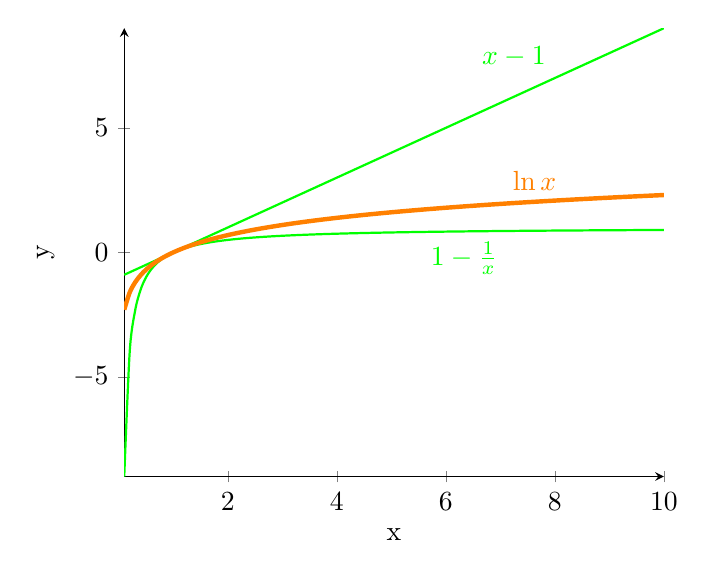
\begin{tikzpicture}[domain=0.1:10]
        \begin{axis} [xlabel = x, ylabel = y, axis lines=left]            \addplot[color=green,samples=100,smooth,thick] {x-1} node[above left,pos=0.8]{$x-1$};
        \addplot[color=green,samples=100,smooth,thick] {1 - 1/x} node[below,pos=0.8]{$1-\frac{1}{x}$};
        \addplot[color=orange,samples=100,smooth,ultra thick] {ln(x)} node[above,pos=0.8]{$\ln{x}$};
        \end{axis}
    \end{tikzpicture}

    \subsection{Upper bound entropia}

    Abbiamo terminato di enunciare le tre proprietà legate all'entropia che ci serviranno nella dimostrazione di alcuni teoremi.
    Vediamo il primo teorema

    \vspace{5px}
    \begin{tcolorbox}
        \textbf{\textcolor{red}{TEOREMA} Upper bound entropia }
        \vspace{5px}
        \begin{center}
            Sia $X$ una variabile casuale che assume $m$ valori distinti $a_1,\dots,a_m$. Allora vale che $H_D(x) \leq \log_D{m}\, \forall D > 1$. Inoltre, $H(X) = \log_D{m}$ se e solo se $X$ ha una distribuzione uniforme su $a_1,\dots,a_m$.
        \end{center}
    \end{tcolorbox}

    \begin{dimo}
        Dimostrare che $H_D(X) \leq \log_D{m}$ equivale a dimostrare che $H_D(X) - \log_D{m} \leq 0$

        $$H_D(x) - \log_D{m} = \somma{m} p_i \log_D{\frac{1}{p_i}} - \log_D{m} \cdot 1$$

        $$= \somma{m} p_i \log_D{\frac{1}{p_I}} - \log_D{m} \cdot \somma{m} p_i$$

        $$= \somma{m} p_i(\log_D{\frac{1}{p_i}} - \log_D{m}) = \somma{m} p_i (\log_D{\frac{1}{p_i\cdot m}})$$
        Applichiamo il cambiamento di base

        $$= \somma{m} p_i (\ln{\frac{1}{m p_i}} \frac{1}{\ln{D}})$$
        Utilizziamo la seconda proprietà che abbiamo enunciato prima

        $$\leq \somma{m} p_i (\frac{1}{m p_i} - 1)(\frac{1}{\ln{D}}) = \frac{1}{\ln{D}} (\somma{m} p_i \frac{1}{p_i m} - \somma{m} p_i)$$

        $$= \frac{1}{\ln{D}} (\somma{m} \frac{1}{m} - \somma{m} p_i) = 0$$
        Dimostriamo ora la seconda parte del teorema. Assumiamo quindi che $P(X = a_i)  = \frac{1}{m} \, \forall i \in 1\dots m$

        $$H_D(X) = \somma{m} \frac{1}{m} \log_D{m} = \log_D{m}$$

    \end{dimo}

    \section{Entropia relativa}

    Introduciamo il concetto di entropia relativa

    $$D(X || Y) = \sum_{s \in S} P_X(s) \log_D{\frac{P_X(s)}{P_Y(s)}}$$
    Notiamo alcune cose

    \begin{itemize}
        \item E' chiamata $D$ perché assomiglia a una distanza, anche se è asimmetrica (ovvero, $D(X || Y) \neq D(Y || X)$). Misura la diversità tra due distribuzioni, $X$ e $Y$.
        \item $S$ è un dominio generico. Deve essere uguale sia per $X$ che per $Y$.
    \end{itemize}


    \vspace{5px}
    \begin{tcolorbox}
        \textbf{\textcolor{red}{TEOREMA} Non negatività entropia relativa}
        \vspace{5px}
        \begin{center}
            Per ogni coppia di variabili casuali $X$ e $Y$ definite su uun dominio comune $S$, vale la disuguaglianza $D(X||Y) \geq 0$.
        \end{center}
    \end{tcolorbox}

    \begin{dimo}
        $$D(X||Y) = \sum_{s \in S} P_X(s) \log_D{\frac{P_X(s)}{P_Y(s)}} = \sum_{s \in S} P_X(s) \ln{\frac{P_X(s)}{P_Y(s)}} \frac{1}{\ln{D}}$$

        $$= \frac{1}{\ln{D}} \sum_{s \in S} P_X(s) \ln{\frac{P_X(s)}{P_Y(s)}} $$
        Per la terza proprietà possiamo scrivere

        $$\geq \frac{1}{\ln{D}} \sum_{s \in S} P_X(s) \frac{P_Y(s)}{P_X(s)} =  \frac{1}{\ln{D}} (\sum_{s \in S} P_X(s) - \sum_{s \in S} P_Y(s)) = 0 $$
    \end{dimo}

    \section{Legame tra valore atteso ed entropia}

    Enunciamo ora un teorema che lega il valore atteso con il concetto di entropia. Questo teorema serve per dare un lower bound al valore atteso. Vedremo quindi che il valore atteso almeno vale quanto l'entropia. Ciò conferma quello che abbiamo detto la lezione scorsa, cioè che l'entropia è il limite inferiore alla correttezza del codice.

    \vspace{5px}
    \begin{tcolorbox}
        \textbf{\textcolor{red}{TEOREMA} Lower bound valore atteso }
        \vspace{5px}
        \begin{center}
            Se $c\, :\, \mathbb{X} \rightarrow \mathbb{D}^+$ è un codice istantaneo $d$-ario per una sorgente \modello , allora vale che

            $$\mathbb{E}[l_c] \geq H_D(X)$$
        \end{center}
    \end{tcolorbox}

    \begin{dimo}
        Sia $Z\,:\, \mathbb{X} \rightarrow \mathbb{R}$ una variabile aleatoria casuale con distribuzione

        $$q(x) = \frac{D^{-l_c(x)}}{\sum_{x' \in \mathbb{X} } D^{-l_c(x')}}$$
        Allora

        $$\va[l_c] - H_D(X) = \values p_x l_c(x) - \values p(x) \log_D{\frac{1}{p_x}} =$$
        $$= \values p(x)(l_c(x) - \log_D{\frac{1}{p(x)}})$$
        Usando il fatto che $1 \cdot l_c(x) = \log_D{D} \cdot l_c(x) = \log_D{D^{l_c(x)}}$ possiamo scrivere

        $$= \values p(x) (\log_D{D^{l_c(x)}} + \log_D{p(x)}) = \values p(x) \log_D{(\frac{p(x)}{D^{-l_c(x)}} \cdot 1)}$$
        Sapendo che $\values \frac{D^{-l_c(x)}}{\sum_{x' \in \mathbb{X}} D^{-l_c(x')}} = 1$ scriviamo

        $$\values p(x) \log_D{(\frac{p_x}{D^{-l_c(x)}} \frac{ \sum_{x' \in \mathbb{X}} D^{-l_c(x')}}{\sum_{x'' \in \mathbb{X}} D^{-l_c(x'')}})}$$

        $$=  \values p(x) (\log_D{(p_x \frac{\sum_{x' \in \mathbb{X} } D^{-l_c(x')}}{D^{-l_c(x)}})}) - \log_D(\values D^{-l_c(x)})$$
        Sappiamo che $\frac{\sum_{x' \in \mathbb{X} } D^{-l_c(x')}} = \frac{1}{q(x)}$

        $$= \values p(x) (\log_D{\frac{p(x)}{q(x)}}) - \values p(x) \log_D{\sum_{x' \in \mathbb{X}} D^{-l_c(x')}}$$
        Considerazioni finali:

        \begin{itemize}
            \item $\values p(x) (\log_D{\frac{p(x)}{q(x)}})$ è l'entropia relativa, che sappiamo essere non negativa.
            \item Prendiamo in considerazione la parte rimanente dell'equazione. Notiamo che $\sum_{x' \in \mathbb{X}} D^{-l_c(x')}$ è $<1$ per la disuguaglianza di Kraft. Il logaritmo di un numero $<0$ è negativo. La sommatoria di numeri negativi è negativa. Siccome davanti c'è un meno diventa tutto positivo.
            \item L'espressione diventa così una somma. La somma di due quantità non negative è essa stessa non negativa. Quindi abbiamo dimostrato il teorema.
        \end{itemize}
    \end{dimo}


    \section{Sardinas-Patterson}

    L'algoritmo di Sardinas-Patterson serve a capire se un codice è univocamente decodificabile o meno.
    Dato un insieme di parole di codice vogliamo quindi capire se formano un codice univocamente decodificabile. L'algoritmo procede come segue:

    \begin{itemize}
        \item Prendiamo l'insieme di parole dato e lo chiamiamo $S_1$
        \item Costruiamo l'insieme $S_2$ in questo modo:
        $$x \in S_1 : xy \in S_1 \rightarrow y \in S_2$$
        Ovvero se $x \in S_1$ è testa di una parola, metto la coda di questa parola nell'insieme $S_2$
        \item Per costruire l'insieme $S_{i+1}$ procedo in questo modo:

        $$x \in S_1 : xy \in S_i \rightarrow y \in S_{i+1}$$

        $$z \in S_i : zy \in S_1 \rightarrow y \in S_{i+1}$$
        \item Ci fermiamo quando o troviamo un insieme vuoto ( e quindi il codice è univocamente decodificabile) oppure quando nell'insieme $S_i$ troviamo una (almeno una) parola del codice (cioè in $S_1$). In questo caso non è univocamente decodificabile.
    \end{itemize}
    Provare a fare i seguenti esercizi:

    \begin{es}
        Il codice $\{A,BCA,DE,CDC,AABC,C\}$ è univocamente decodificabile?
    \end{es}

    \begin{es}
        Il codice $\{A,E,C,ABB,CED,BBEC\}$ è univocamente decodificabile?
    \end{es}

    \chapter{Lezione V}
    \label{cap:Lezione V}
    \section{Upper bound valore atteso}

    Sappiamo che $H_D(X) \leq \va [l_c]$, ma non sappiamo quanto siano vicini. La lunghezza media potrebbe essere molto distante, ciò renderebbe il codice poco efficiente.
    Sia \modello il modello sorgente, con $\mathbb{X} = \{x_1,\dots,x_m\}$ e $p = \{p_1,\dots,p_m\}$ vale il seguente teorema

    \vspace{5px}
    \begin{tcolorbox}
        \textbf{\textcolor{red}{TEOREMA} Upper bound valore atteso}
        \vspace{5px}
        \begin{center}
            Dato il codice istantaneo $c$ di Shannon, con lunghezze $l_i = l_c(x_i)$ tale che $l_i = \lc \log_D{\frac{1}{p_i}} \rc \, \forall i \in 1,\dots,m$, allora

            $$\va [l_c] < H_D(x) + 1$$
        \end{center}
    \end{tcolorbox}

    \begin{dimo}
        $$\va[l_c] = \somma{m} p_i \lc \log_D{\frac{1}{p_i}} \rc < \somma{m} p_i (\log_D{\frac{1}{p_i}} + 1)$$
        $$= \somma{m} p_i \log_D{\frac{1}{p_i}} + \somma{m} p_i = H_D(X) + 1$$
    \end{dimo}
    \noindent
    Questo teorema ci dice che al massimo spreco un bit per simbolo rispetto all'ottimo.
    Questo sembra un buon risultato, però se il messaggio è lungo (cioè ha tanti simboli) perderemo tanti bit.

    \begin{defi}
        L'inefficienza cresce linearmente con la lunghezza del messaggio.
    \end{defi}

    \noindent
    Dati $c\, :\, \mathbb{X} \rightarrow \mathbb{D}^+$ e $C\, :\, \mathbb{X}^+ \rightarrow \mathbb{D}^+$ definiamo l'estrazione a blocchi di $n$. Vale il seguente fatto

    $l_c(x_1,\dots,x_n) \geq l_{c_n} (x_1,\dots,x_n)$
    Cioè la lunghezza di un messaggio dove i simboli sono trattati singolarmente è non minore della lunghezza del messaggio in cui sono trattati come blocchi.
    Infatti

    $$l_c(x_1,\dots,x_n) = \somma{n} \lc \log_D{\frac{1}{p_i}}\rc \geq  \lc \somma{n}  \log_D{\frac{1}{p_i}} \rc$$
    $$= \lc \log_D{\frac{1}{\prod_i p_i}} \rc  =
    \lc \log_D{\frac{1}{p(x_1,\dots,x_n)}} \rc  = l_{c_n} (x_1,\dots,x_n)$$
    Dove

    $$C_n \, :\, \mathbb{X}^n \rightarrow \mathbb{D}^+$$
    Quindi sostituiamo la giustapposizione di $n$ simboli con l'estrazione di un messaggio da $n$ simboli. In questo modo paghiamo $1$ bit per ogni $n$ simboli. Abbiamo quindi un nuovo modello sorgente, \nmodello, che è più complesso!

    \noindent
    A questo punto ci chiediamo se esiste una relazione tra $H(x_1,\dots,x_n)$ e $H(x)$.
    Cominciamo con scrivere la definizione di $H(x_1,\dots,x_n)$, ovvero

    $$H(x_1,\dots,x_n) = \sum_{x_1,\dots,x_n} p_n(x_1,\dots,x_n) \log_D{\frac{1}{p_n(x_1,\dots,x_n)}}$$
    Sappiamo che $p_n(x_1,\dots,x_n) = \prod_i P(x_i)$ e anche che

    $$\log_2{\frac{1}{\prod_{i=1}^n p(x_i)}} = \log_2 \prod p(x_i)^{-1} $$
    $$= \somma{n} \log_2 p(x_i)^{-1} = \somma{n} \log_2 \frac{1}{p(x_i)}$$
    Quindi riprendiamo l'equazione di prima e applichiamo la definizione soprastante

    $$\sum_{x_1} \dots \sum_{x_n} \prod_{i = 1}^n p(x_i) \cdot \somma{n} \log_2{\frac{1}{p(x_i)}}$$
    Per capire come procedere analizziamo il caso $n=2$.

    $$\sum_{x_1} \sum_{x_2} \prod_{i=1}^2 p(x_i) (\log_2{\frac{1}{p_1}} + \log_2{\frac{1}{p_2}}) $$
    $$ = \sum_{x_1} \sum_{x_2} \log_2{\frac{1}{p_1}} p_1 p_2 +  \log_2{\frac{1}{p_2}} p_2 p_1$$

    $$=  \sum_{x_1} \sum_{x_2} p(x_1) p(x_2) \log_2{\frac{1}{p(x_1)}} +  \sum_{x_1} \sum_{x_2} p(x_1) p(x_2) \log_2{\frac{1}{p(x_2)}} = $$

    $$= \sum_{x_1} p(x_1) \log_2{\frac{1}{p(x_1}} \sum_{x_2} p(x_2) + \sum_{x_2} p(x_2) \log_2{\frac{1}{p(x_2}} \sum_{x_1} p(x_1)$$

    $$= H(x_1) + H(x_2)$$
    In generale possiamo quindi affermare che

    $$H(x_1,\dots,x_n) = n H(x)$$

    \section{Primo teorema di Shannon}
    Siamo pronti per enunciare il primo teorema di Shannon che avevamo accennato nella prima lezione.


    \vspace{5px}
    \begin{tcolorbox}
        \textbf{\textcolor{red}{TEOREMA} Primo teorema di Shannon}
        \vspace{5px}
        \begin{center}
            Sia  $\mathbb{C}_n \, :\, \mathbb{X}^N \rightarrow \mathbb{D}^+$ un codice di Shannon d-ario a blocchi per la sorgente \modello, ossia $l_{\mathbb{C}_n} (\listina{x}{n}) = \lc \myLog{D}{p(\listina{x}{n})} \rc$  allora

            $$\lim_{n\rightarrow + \infty} \frac{1}{n} \va[l_c] = H_D(X)$$
        \end{center}
    \end{tcolorbox}

    \begin{dimo}
        Sappiamo che
        $$H_D(\listina{x}{n}) = n H(X) \leq \va[l_c] < H_D(\listina{x}{n}) = n H(X) + 1 $$
        Dividendo tutto per $n$ otteniamo

        $$H(x) \leq \frac{1}{n} \va[l_c] < H(X) + \frac{1}{n}$$
        Se $n \rightarrow + \infty$ allora $H(X) = H(X) + \frac{1}{n}$ e quindi  $\va[l_c] = H(X)$
    \end{dimo}

    \noindent
    Il teorema precedente ci indica che il valore atteso si "schiaccia" sull'entropia col crescere della dimensione dei blocchi. Quindi se facciamo crescere la dimensione del blocco paghiamo poco in termini di bit!

    \section{Approssimare il modello}
    Purtroppo non conosciamo a propri il modello \modello e quindi ne dobbiamo fare una stima

    $$<\!\mathbb{Y},q\!>$$
    L'entropia relativa $D(X||Y)$ ci dice l'errore pagato quando si usa la stima $\mathbb{Y}$ per \sorgente.
    Vale il seguente teorema:

    \vspace{5px}
    \begin{tcolorbox}
        \textbf{\textcolor{red}{TEOREMA} Valore atteso ed entropia relativa}
        \vspace{5px}
        \begin{center}
            Dato il modello sorgente \modello, se $c\,:\,\mathbb{X} \rightarrow \mathbb{D}^+$ è codice di Shannon con $l_c(x) = \lc \myLog{D}{q(x)} \rc$, dove $q$ è una distribuzione su $x$, allora

            $$\va[l_c] < H_D(x) + 1 + D(X||Y)$$
        \end{center}
    \end{tcolorbox}

    \begin{dimo}
        $$\va[l_c] = \sum_{x \in \mathbb{X}} p(x) \lc \myLog{D}{q(x)} \rc < \sum_{x \in \mathbb{X}} p(x) (\myLog{D}{q(x)} + 1)$$
        $$= \sum_{x \in \mathbb{X}} p(x) \myLog{D}{q(x)} + \sum_{x \in \mathbb{X}} p(x) = \sum_{x \in \mathbb{X}} p(x) \log_D{(\frac{1}{q(x)} \frac{p(x)}{p(x)})} + 1$$

        $$= \sum_{x \in \mathbb{X}} p(x) \log_D{\frac{p(x)}{q(x)}} + \sum_{x \in \mathbb{X}} p(x) \myLog{D}{p(x)} + 1$$
        $$= D(X || Y) + H_D(X) + 1$$
    \end{dimo}


    \chapter{Lezione VI}


    \section{Algoritmo di Huffman}

    In questa lezione presentiamo un algoritmo per la costruzione di un codice di Huffman, con $D > 1$.

    \begin{enumerate}
        \item Ordina i simboli sorgente in base alla probabilità.
        \item Crea modello sorgente fittizia in cui i $D$ simboli meno probabili vengono raggruppati e sostituiti con un nuovo simbolo. La sua probabilità è pari alla somma delle probabilità dei simboli che sostituisce.
        \item Se la sorgente contene più di $D$ simboli ripeti il procedimento.
    \end{enumerate}
    Dato il modello \modello con $|\mathbb{X}| = m$, l'algoritmo termina quando

    $$|\mathbb{X}| = (D-1)k + 1$$
    dove $k$ indica l'iterazione. Ovvero, rimuoviamo k volte $d-1$ simboli, se ne resta $1$ solo abbiamo terminato. Se non esiste questo $k$ allora aggiungiamo dei simboli "dummy" con probabilità pari a $0$.

    \newpage
    \section{Codici di Huffman}

    Presentiamo adesso un teorema che lega ci permette di capire se i codici di Huffman siano buoni o meno.

    \begin{tcolorbox}
        \textbf{\textcolor{red}{TEOREMA} Relazione tra codice di Huffman e qualsiasi altro codice}
        \vspace{5px}
        \begin{center}
            Data una sorgente \modello e dato $D > 1$, il codice $D$-ario $c$ di Huffman minimizza $\va[l_c]$ tra tutti i codici istantanei per la medesima sorgente. Ovvero,

            $$\va[l_c] \leq \va[l_{c',c_2,\tilde c}]$$
        \end{center}
    \end{tcolorbox}

    \noindent
    Per dimostrare il teorema ci serve prima enunciare un fatto.

    \vspace{5px}
    \begin{tcolorbox}
        \textbf{\textcolor{red}{FATTO} }
        \vspace{5px}
        \begin{center}
            Sia $c'$ un codice $D$-ario di Huffman per la sorgente $\mathbb{X}' \,=\, \{\listina{x}{m-d+1}\}$ con probabilità $p_1 \geq \dots \geq p_{m-d+1}$. Sia \sorgente la sorgente ottenuta togliendo da $\mathbb{X}'$ il simbolo $x_k$ e aggiungendo $d$ nuovi simboli, $x_{m-d+2} \dots x_{m+1}$, con probabilità $p_{m-d+2},\dots,p_{m+1}$, tali che $p(.) > 0$ e anche che $p(.) < p_{m-d+1}$. Inoltre deve valere che $p_{m-d+2} + \dots + p_{m+1} = p_k$.
            Allora vale che

            $$ c(x) = \begin{cases}
                          c'(x)\hfill \;\text{se}\;x\neq x_k \\
                          c'(x_k) \cdot i \hspace{40px} \; \text{se} \; x = x_{m-d+2} \; \text{a} \; x_{m+1} \forall i \in 0,\dots,d-1
            \end{cases}$$
            è un codice di Huffman per la sorgente.
        \end{center}
    \end{tcolorbox}

    \noindent
    Il fatto esposto è l'algoritmo di Huffman proposto "al contrario".
    Dimostriamo ora il teorema.

    \begin{dimo}
        Dimostrazione per induzione.

        \vspace{5px}

        \noindent
        $m=2$, caso base.

        \vspace{5px}

        \noindent
        Per costruzione, Huffman produce il codice $c(x_1) = 0$ e $c(x_2) = 1$ che è ottimo, qualunque sia la distribuzione di probabilità.

        \vspace{5px}

        \noindent
        Ipotesi induttiva: Huffman ottimo per $k\leq m-1$

        \vspace{5px}

        \noindent
        Fissiamo \modello (con $m$ simboli) con $\mathbb{X} = \{\dots,u,\dots,v\}$ dove $p(u)$ e $p(v)$ sono minime. Definiamo  $<\! \mathbb{X}',p'\!>$ con $u,v \in \mathbb{X}$ rimpiazzati da $z \in \mathbb{X}'$.  Inoltre $p'$ è tale che

        $$ p' = \begin{cases}
                    p(x) \hfill \;\text{se}\;x\neq z \\
                    p(u)+p(v) \hspace{40px} \; \text{se} \; x = z
        \end{cases}$$
        Sia $c'$ il codice di Huffman per $<\! \mathbb{X}',p'\!>$. Dato che $|\mathbb{X}'| = m-1$, $c'$ è ottimale per ipotesi induttiva.

        \noindent
        Il codice $c$ per \sorgente è definito come

        $$ c = \begin{cases}
                   c'(x) \hfill \;\text{se}\;x \notin \{u,v\}\\
                   c'(z) \cdot 0 \hspace{40px} \; \text{se} \; x = u \\
                   c'(z) \cdot 1 \hspace{40px} \; \text{se} \; x = v
        \end{cases}$$
        Dimostriamo che $c$ sia ottimo. Innanzitutto vale quanto segue

        $$\va[l_c] = \sum_{x \in \mathbb{X}} l_c(x) p(x)$$
        Esprimiamo il valore atteso in termini di $\mathbb{X'}$, quindi

        $$= \sum_{x \in \mathbb{X}'} l_{c'}(x) p'(x) - l_{c'}(z) p'(z) + l_c(u) p(u) + l_c(v) p(v) $$

        $$= \va[l_{c'}] - l_{c'}(z) p'(z) + (l_{c'}(z) + 1)p(u) + (l_{c'}(z) +1) p(v)$$
        Raggruppiamo per $l_{c'}(z) + 1$

        $$= \va[l_{c'}] - l_{c'}(z) p'(z) + (l_{c'}(z) + 1)(p(u) + p(v))$$
        Sapendo che $p(u) + p(v) = p'(z)$

        $$= \va[l_{c'}] - l_{c'}(z) p'(z) + l_{c'}(z) p'(z) + p'(z)$$

        $$= \va[l_{c'}] + p'(z)$$
        Per dimostrare l'ottimalità di $c$ consideriamo un altro codice $c_2$ per \modello e verifichiamo che $\va[l_c] \leq \va[l_{c_2}]$

        \noindent
        Sia $c_2$ istantaneo per \modello. Siano $r,s \in \mathbb{X}$ tali che $l_{c_2} (r)$ e $l_{c_2}(s)$ sono massimi. Senza perdità di generalità possiamo assumere che $r,s$ siano fratelli nell'albero di codifica $c_2$. Infatti,

        \begin{itemize}
            \item  se non fossero fratelli e avessero un altro fratello (es. $s$ ha fratello $f$) allora scegliamo $s$ e $f$ invece che $s$ e $r$.
            \item  Se non avessero fratelli possiamo sostituire le loro codifiche con quelle del padre fino a riportarci in una situazione in cui abbiano un fratello.
        \end{itemize}

        \noindent
        Definiamo ora il codice $\tilde c_2$.

        $$ \tilde c_2 = \begin{cases}
                            c_2(x) \hspace{40px} \;\text{se}\;x \notin \{u,v,r,s\}\\
                            c_2(u)  \hfill \; \text{se} \; x = r \\
                            c_2(r)  \hfill \; \text{se} \; x = u \\
                            c_2(v)  \hfill \; \text{se} \; x = s \\
                            c_2(s)  \hfill \; \text{se} \; x = v
        \end{cases}$$
        Dove scambiamo la codifica di $r$ con quella di $u$ e quella di $s$ con quella di $v$.

        \vspace{5px}

        \noindent
        Esaminiamo la differenza tra $c_2$ e $\tilde c_2$

        $$\va[l_{\tilde c_2}] - \va[l_{c_2}] = $$

        \begin{align*}
            = p(r)l_{c_2}(u) + p(u) l_{c_2}(r) + p(s) l_{c_2}(v) + p(v) l_{c_2}(s) - p(u)l_{c_2}(u) \\ - p(r) l_{c_2}(r) - p(v) l_{c_2}(v) - p(s) l_{c_2}(s)
        \end{align*}

        \begin{align*}
            = p(r) [l_{c_2}(u) - l_{c_2}(r)] - p(u)[l_{c_2}(u) - l_{c_2}(r)] + p(s) [l_{c_2}(v) - l_{c_2}(s)]\\ - p(v)[l_{c_2}(v) - l_{c_2}(s)]
        \end{align*}

        $$[p(r) - p(u)] [l_{c_2}(u) - l_{c_2}(r)] + [p(s) - p(v)] [l_{c_2}(v) - l_{c_2}(s)]$$
        Sapendo che
        \begin{itemize}
            \item $p(r) - p(u) \geq 0$, dato che $u$ è minimo, insieme a $v$.
            \item $l_{c_2}(u) - l_{c_2}(r) \leq 0$
            \item  $p(s) - p(v) \geq 0$, dato che $v$ è minimo, insieme a $u$.
            \item $l_{c_2}(v) - l_{c_2}(s) \leq 0$
        \end{itemize}
        Possiamo affermare che

        $$\va[l_{\tilde c_2}] - \va[l_{c_2}] \leq 0$$
        Quindi

        $$\va[l_{\tilde c_2}] \leq \va[l_{c_2}] $$


    \end{dimo}


    \chapter{Lezione VII}

    \section{Termine dimostrazione lezione VI}
    Introduciamo il codice $c_2'$, fatto come segue

    $$ \tilde c_2' = \begin{cases}
                         \tilde c_2(x) \hspace{40px} \;\text{se}\;x \neq z\\
                         \omega  \hfill \; \text{se} \; x = z \\
    \end{cases}$$
    Dove $c_2'$ è definito sulla sorgente $<\! \mathbb{X}',p'\!>$. Inoltre, dopo avere scambiato $r$ e $s$ con $u$ e $v$, quest'ultimi sono fratelli. Quindi

    \begin{itemize}
        \item $\tilde c_2 (u) = \omega \cdot 0$
        \item $\tilde c_2 (v) = \omega \cdot 1$
    \end{itemize}
    Allora,

    $$\va[l_{\tilde c_2}] = \sum_{x \in \mathbb{X}': x \neq z} p'(x) l_{\tilde c_2}(x) + p(u) (l_{c_2'} (z) + 1) + p(v) (l_{ c_2'}(z) +1)$$

    $$= \sum_{x \in \mathbb{X}': x \neq z} p'(x) l_{\tilde c_2}(x) + p'(z) l_{c_2'}(z) + p'(z)$$

    $$= \va[l_{c_2'}] + p'(z) \geq \va[l_{c'}] + p'(z)$$
    Mettendo tutto insieme

    $$\va[l_c] = \va[l_{c'}] + p'(z) \leq \va [l_{c_2'}] + p'(z)  = \va[l_{\tilde c_2}] \leq \va[l_{c_2}]$$

    $$\va[l_c] \leq  \va[l_{c_2}] $$

    \section{Disuguaglianza di Kraft-McMillan}
    Per cercare il codice ottimo ci siamo ristretti ai soli codici istantanei. Così facendo rischiamo, però, di lasciare fuori codici che potrebbero essere ottimi, nonostante non siano istantanei.

    In realtà questi codici non esistono, dato che anche i codici univocamente decodificabili seguono la disuguaglianza di Kraft.

    \vspace{5px}
    \begin{tcolorbox}
        \textbf{\textcolor{red}{Teorema} Disuguaglianza di Kraft-McMillan }
        \vspace{5px}
        \begin{center}

            $\listina{l}{m}$ sono le lunghezze di un codice $D$-ario univocamente decodificabile, per una sorgente di $m$ simboli, se e solo se

            $$\somma{m} D^{-l_i} \leq 1$$

        \end{center}
    \end{tcolorbox}
    Prima di dimostrare il teorema definiamo l'estensione $k$-esima, $\mathbb{C}_k$, di un codice $c$,

    $$\mathbb{C}_k \, : \, \mathbb{X}^k \rightarrow \mathbb{D}^+$$

    \begin{dimo}
        Per dimostrare che $\somma{m} D^{-l_i} \leq 1$ implica che il codice sia univocamente decodificabile notiamo che, se vale $\somma{m} D^{-l_i} \leq 1$, allora $\listina{l}{m}$ sono lunghezze di un codice istantaneo, quindi di un codice univocamente decodificabile.

        \vspace{5px}

        \noindent
        Dimostriamo l'altro lato, ovvero che dato un codice univocamente decodificabile vale la disuguaglianza.
        $\forall k \geq 1$ possiamo scrivere

        $$(\sum_{x \in \mathbb{X}} D^{-l_c(x)})^k = \sum_{x_1} \dots \sum_{x_k} D^{-l_c(x_1)} \dots D^{-l_c(x_k)} = (1)$$
        Questo è verifcabile provando il caso $k=2$

        $$(\sum_i a_i)^2 = (\sum_i a_i) (\sum_j a_j) = \sum_i \sum_j a_i a_J $$

        $$(1) = \sum_{(\listina{x}{k}) \in \mathbb{X}^k} D^{-(l_c(x_1) + \dots + l_c(x_k))} =  \sum_{(\listina{x}{k}) \in \mathbb{X}^k} D^{-l_{\mathbb{C}_k} (\listina{x}{k})} = (2)$$
        Dove

        $$l_{\mathbb{C}_k} (\listina{x}{k}) = l_c(x_1) + \dots + l_c(x_k)$$
        Introduciamo l'insieme $\mathbb{X}_n^k$, definito come segue

        $$\{(\listina{x}{k}) \in \mathbb{X}^k : l_{\mathbb{C}_k} (\listina{x}{k}) = n \}$$
        Quindi,

        $$(2) = \sum_{(\listina{x}{k}) \in \mathbb{X}^k} D^{-l_{\mathbb{C}_k} (\listina{x}{k})} = \sum_{n = 1}^{k \cdot l_{max}} \sum_{(\listina{x}{k}) \in \mathbb{X}_n^k} D^{-l_{\mathbb{C}_k} (\listina{x}{k})}$$

        $$= \sum_{n = 1}^{k \cdot l_{max}}  |\mathbb{X}_n^k|D^{-n} = (3)$$
        Siccome $c$ è univocamente decodificabile, $\mathbb{C}$ è iniettiva. Quindi $|\mathbb{X}_n^k| \leq |D^n|$

        $$ (3) \leq \sum_{n = 1}^{k \cdot l_{max}} D^n D^{-n}  \leq k \cdot l_{max}$$
        Allora,

        $$(\sum D^{-l_c(x)})^k \leq k l_{max}$$
        Poniamo ora $\sum D^{-l_c(x)} = M$ e ci chiediamo quanto valga $M$.

        \begin{tikzpicture}[domain=-0.5:2]
            \begin{axis} [xlabel = x, ylabel = y, axis lines=center,  yticklabel=\empty, xticklabel = \empty]            \addplot[color=color,samples=100,smooth,ultra thick] {2^x} node[above left,pos=0.80] {$M^x\, M > 1$};

            \addplot[color=greenie,samples=100,smooth,ultra thick] {0.5^x} node[above right,pos=0.60] {$M^x\, 0 < M \leq 1$};
            \addplot[color=blue,samples=100,smooth,ultra thick] {x*1.4} node[below right,pos=0.80] {$x \cdot l_{max}$};
            \end{axis}
        \end{tikzpicture}

        \noindent
        Siccome vogliamo che $M^x$ sia sotto $x \cdot l_{max}$, allora $M$ deve essere compreso tra $0$ e $1$, possiamo concludere che

        $$(\sum D^{-l_c(x)})^k \leq 1$$

    \end{dimo}

    \chapter{Lezione VIII}

    \section{Esercizi di probabilità}

    \begin{es}
        Sapendo che la probabilità di un messaggio
        di essere corrotta è $\frac{1}{8}$, quanti bit mi servono per rappresentarla?
        Usiamo la formula
        $$\log_2{\frac{1}{p_i}}$$
        Dato che $p_i = \frac{1}{8}$ allora ci serviranno
        $$\log_2{8} = 3$$
        bit.
    \end{es}

    \begin{es}
        Qual è la probabilità di ottenere $4$ messaggi dove il primo è corretto e gli altri $3$ no, sapendo che $p = \frac{1}{8}$ ($p$ è la probabilità che il messaggio sia corretto)?

        $$\frac{1}{8} (1 - \frac{1}{8})^3$$

    \end{es}

    \begin{es}
        Preso l'esercizio precedente, quanti bit ci servono?

        $$\log_2{\frac{1}{8} (1 - \frac{1}{8})^3} = \log_2{\frac{1}{8}} + \log_2{(1 - \frac{1}{8})^3} = -3 + \log_2{(1-\frac{1}{8})^3}$$
    \end{es}

    \begin{es}
        Abbiamo un dado a $6$ facce lanciato $20$ volte. Qual è la probabilità  di...

        \begin{itemize}
            \item Fare $20$ lanci e il $5$ non esce mai?
            $$(\frac{5}{6})^{20}$$
            \item Fare $20$ lanci e il $5$ esce una volta?
            $$(\frac{5}{6})^{19}\cdot(\frac{1}{6})\cdot20$$
            \item  Fare $20$ lanci ed esce almeno $1$ volta il $5$? E' come chiedersi la probabilità opposta a quando non esce mai il $5$ quindi:

            $$1 - P(\text{non esce mai 5}) = 1 - (\frac{5}{6})^{20}$$
        \end{itemize}
    \end{es}

    \section{Numero di bit necessari}
    Quanti bit ci servono per comunicare il risultato di un certo evento? Se usiamo un codice istantaneo...

    $$H(x) <\,\text{n° bit}$$
    E se abbiamo 2 variabli, ovvero 2 risultati da comunicare?

    $$H(X,Y) = \sum_{x \in \mathbb{X}} \sum_{y \in \mathbb{Y}} p(x,y) \log{\frac{1}{p(x,y)}}$$
    $H(X,Y)$ è detta \textbf{entropia congiunta}.
    Quanti bit ci servono avendo un evento condizionante? Cioè, se il ricevente conosce $\mathbb{X}$, quanti bit ci servono per comunicare $\mathbb{Y}$?

    $$H(Y|X) = \sum_{x \in \mathbb{X}} p(x) H(\mathbb{Y} | \mathbb{X} = x)$$
    $$= \sum_{x \in \mathbb{X}} p(x) (\sum_{y \in \mathbb{Y}} p(y|x) \myLog{2}{p(y|x)})$$
    $$= \sum_{x \in \mathbb{X}} \sum_{y \in \mathbb{Y}} p(x,y) \myLog{2}{p(y|x)} $$
    $H(Y|X)$ è detta \textbf{entropia condizionata}. Seguono due definizioni di probabilità

    \begin{defi}
        $p(x,y)$ è detta \textbf{probabilità congiunta}, ed è la probabilità che avvenga sia $x$ che $y$.
    \end{defi}
    \begin{defi}
        $p(x) = \sum_{y \in \mathbb{Y}} p(x,y)$ è detta \textbf{probabilità marginale}.
    \end{defi}
    \begin{defi}
        $p(y|x) = \frac{p(x,y)}{p(x)}$ è detta \textbf{probabilità condizionale}.
    \end{defi}



    \vspace{5px}
    \begin{tcolorbox}
        \textbf{\textcolor{red}{FATTO} Chain Rule per l'entropia}
        \vspace{5px}
        \begin{center}
            Vale la seguente uguaglianza
            $$H(x,y) = H(x) + H(y|x) = H(y) + H(x|y)$$
            Inoltre vale anche la seguente per gli spazi condizionati
            $$H(x,y|z) = H(x,z) + H(y|x,z)$$

        \end{center}
    \end{tcolorbox}

    \section{Esercizi su entropia}

    \begin{es}
        Sia $x \in X$ una variabile rappresentante l'estrazione di un numero tra $0$ e $9$, e $y$ definita come $y= x+2 \mod 10$, quanto vale $H(Y|X)$? Vale $0$! Infatti, se il ricevente ha gia $X$ non dobbiamo inviare alcuna informazione. Il ricevente può calcolarsi $Y$ da solo.
    \end{es}

    \begin{es}
        Sia $X = \{-1,0,1\}$ e $Y = X^2$, quanto vale $H(Y|X)$?  Vale $0$ per la stessa ragione di prima. E invece $H(X|Y)$ ? Sicuramente è $\neq 0 $. Non possiamo ricavare $X$ avendo solo $Y$.
    \end{es}

    \begin{es}
        Dato un sistema $S\!-\!C-\!R$ (sorgente-canale-ricevente). Sia $M$ una matrice che rappresenta il canale
        \[\mathbf{M} =
        \bordermatrix{ & b_1 & b_2 & b_3 & b_4 & b_5 \cr
        a_1 & 0.3 & 0.1 & 0.3 & 0.1 & 0.1 \cr
        a_2 & 0.2 & 0.2 & 0.2 & 0.2 & 0.2 \cr
        a_3 & 0.3 & 0.3 & 0.1 & 0.1 & 0.2  \cr
        a_4 & 0.3 & 0.3 & 0.3 & 0.05 & 0.05} \qquad
        \]
        e $\mathbb{X} = \{a_1,\dots,a_4\}$ e $p =[0.2, 0.2, 0.2, 0.4]$. Calcoliamo $H(R|S)$:

        $$H(R|S) = \sum_{i = 1}^4 p(a_i) H(R|a_i)$$
        $$= \sum_{i = 1}^4 p(s_i) \sum_{j = 1}^5 p(b_j|a_i) \cdot \log_2{\frac{1}{p(b_j|a_i)}}$$
        E' giusto? No! Non abbiamo conteggiato che:
        \begin{enumerate}
            \item La somma dei $p(a_i)$ sia $= 1$.
            \item La somma delle righe della matrice è uguale a $1$.
        \end{enumerate}
        La prima riga della matrice dato non fa $1$!
    \end{es}


    \begin{es}
        Stesso esercizio di prima ma...
        \[ M =
        \begin{bmatrix}
            0.2 & 0.2 & 0.3 & 0.2 & 0.1  \\
            0.2 & 0.5 & 0.1 & 0.1 & 0.1 \\
            0.6 & 0.1 & 0.1 & 0.1 & 0.1 \\
            0.3 & 0.1 & 0.1 & 0.1 & 0.4
        \end{bmatrix}
        \]
        con $p = [0.2, 0.3, 0.1, 0.4]$. Calcolare $H(R|S)$. Stessa formula di prima, troviamo il risultato dei componenti!
        $$H(R|a_1) = \sum_{j = 1}^5 p(b_j|a_1) \log_2{\frac{1}{p(b_j|a_1)}} = 2.246$$
        In modo analogo calcoliamo gli altri valori

        $$H(R|a_2) = 1.96095$$

        $$H(R|a_3) = 1.77$$

        $$H(R|a_4) = 2.046 $$
        Quindi

        $$H(R|S) = \sum_{i=1}^4 p(a_i) H(R|a_i)$$
        $$= (0.2 \cdot 2.246) + (0.3 \cdot 1.96) + (0.1 \cdot 1.77) + (0.4 \cdot 2.046) = 2.033$$

    \end{es}

    \begin{es}
        Esercizio lasciato al lettore (prof. potrebbe chiedere un'idea all'esame).
        Posso ottenere lo stesso risultato in un altro modo? (usando le formule viste prima). Due strade consigliate:

        \begin{itemize}
            \item Usare chain rule
            \item Usare l'uguaglianza
            $$H(S,R) = H(S|R) + H(R) = H(R|S) + H(S)$$
            per trovare e calcolare $H(R|S)$, quindi

            $$H(R|S) = H(S|R) + H(R) - H(S)$$
        \end{itemize}
    \end{es}

    \chapter{Lezione IX}

    \section{Informazione mutua}

    Introduciamo il concetto di \textbf{informazione mutua}. Per informazione mutua si intende un parametro (o misurazione) che fa riferimento a $2$ variabili casuali; Ci dice quanta informazione viene rilasciata da una rispetto all'altra. L'infrmazione mutua è formalmente definita come


    $$I(X,Y) = \sum_{x \in \mathbb{X}} \sum_{y \in \mathbb{Y}} p(x,y) \log{\frac{p(x,y)}{p(x)p(y)}}$$


    \vspace{5px}
    \begin{tcolorbox}
        \textbf{\textcolor{red}{Fatto} Non negatività informazione mutua}
        \vspace{5px}
        \begin{center}

            L'informazione mutua è non negativa, ovvero
            $$I(X,Y) \geq 0$$

        \end{center}
    \end{tcolorbox}

    \begin{dimo}
        Applichiamo la definizione di probabilità congiunta

        $$I(X,Y) = \sum_{x \in \mathbb{X}} \sum_{y \in \mathbb{Y}} p(x,y) \log{\frac{p(y) p(x|y)}{p(x)p(y)}}$$

        $$=\sum_{x \in \mathbb{X}} \sum_{y \in \mathbb{Y}} p(x,y) \log{\frac{1}{p(x)}} + \sum_{x \in \mathbb{X}} \sum_{y \in \mathbb{Y}} p(x,y) \log{p(x|y)}$$

        $$H(X) - H(X|Y) \geq 0$$
    \end{dimo}

    \begin{es}
        Quanto vale l'informazione mutua tra $X$ e $Y$ se sono indipendenti?

        $$H(X|Y) = H(X)$$
        quindi

        $$I(X,Y) = H(X) - H(X) = 0$$
    \end{es}

    \begin{es}
        Quanto vale l'informazione mutua tra $X$ e $Y$ se $X = g(Y)$?
        In questo caso $H(X|Y) = 0$, quindi

        $$I(X,Y) = H(X)$$
    \end{es}

    L'informazione mutua la possiamo esprimere in modi diversi:

    $$ \begin{cases}
           H(Y) = H(Y|X) + I(X,Y)\\
           H(X) = H(X|Y) + I(X,Y) \\
           H(X,Y) = H(X) + H(Y) - I(X,Y) \\
           H(X,Y) = H(X|Y) + H(Y|X) + I(X,Y)
    \end{cases}$$

    \begin{center}

        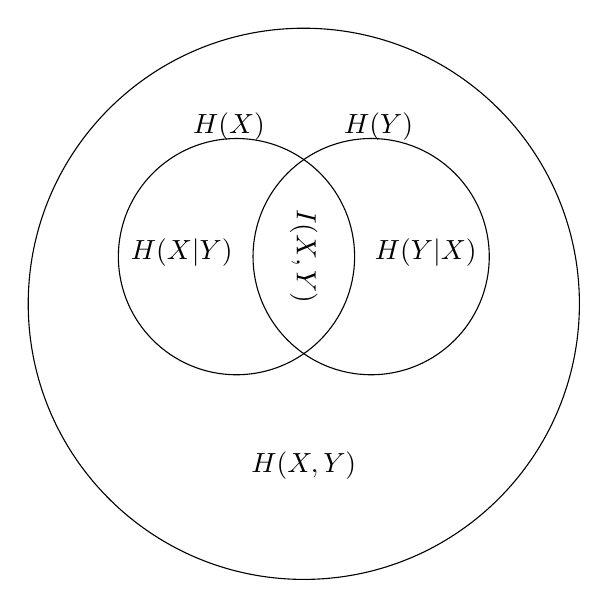
\begin{tikzpicture}
            \node[rotate= -90] at (0, 2.35) {$I(X,Y)$};
            \node[] at (-0.95, 4) {$H(X)$};
            \node[] at (0.95, 4) {$H(Y)$};
            \node[] at (-1.55,2.40) {$H(X|Y)$};
            \node[] at (1.55,2.40) {$H(Y|X)$};

            \draw (90:1.75cm) circle (3.5cm) node[text=black,below, pos =0.8] {$H(X,Y)$};

            \draw (110:2.5cm) circle (1.5cm);
            \draw (70:2.5cm) circle (1.5cm);
        \end{tikzpicture}
    \end{center}
    Vale anche che

    $$I(X,Y|Z) = \sum p(x,y|z) \log{\frac{p(x,y|z)}{p(y|z) p(x|z)}}$$



    \section{Data processing inequality}
    Introduciamo il seguente teorema, che non dimostriamo,

    \vspace{5px}
    \begin{tcolorbox}
        \textbf{\textcolor{red}{Teorema} Data processing inequality}
        \vspace{5px}
        \begin{center}

            Siano $X$,$Y$ e $Z$ variabili casuali s ominio finito tali che $p(x,y,z)$ soddisfa $p(x,y|z) = p(x|y) p(z|y) \forall x,y,z$ (cioè $x$ e $z$ sono indipendenti dato $y$), allora l'informazione mutua tra $x$ e $y$ è $\geq$ dell'informazione mutua tra $x$ e $z$ ovvero
            $$I(X,Y) \geq I(X,Z)$$

        \end{center}
    \end{tcolorbox}

    \vspace{5px}
    \begin{tcolorbox}
        \textbf{\textcolor{red}{Corollario} }
        \begin{center}
            Vale la seguente disequazione:
            $$I(X,Y) \geq I(X,Y|Z)$$
        \end{center}
    \end{tcolorbox}


    \begin{exmp}
        Consideriamo due variabili casuali $X$ e $Y$ bernoulliane indipendenti di parametro $\frac{1}{2}$ e definiamo $Z = X+Y$. Chiaramente $X,Z$ non sono indipendenti dato $Y$. Osserviamo che  $I(X,Y) = 0$ (perché sono indipendenti) mentre

        $$I(X,Y|Z) = H(X|Z) - H(X|Y,Z)$$
        Sappiamo che $H(X|Y,Z) = 0$ quindi
        $$= p(Z = 0) H(X|Z = 0) + p(Z = 1) H(X|Z = 1) + p(Z = 2) H(X|Z = 2)$$
        Dove $p(Z = 0) H(X|Z = 0) = 0$ e $p(Z = 2) H(X|Z = 2) = 0$ allora possiamo scrivere

        $$= p(Z = 1) H(X|Z = 1)$$
        L'entropia di $X$ è massima se $Z = 1$ e allora $H(X|Z = 1) = 1$,
        $$= p(Z = 1) = \frac{1}{2}$$
        Abbiamo quindi costruito un esempio in cui $I(X,Y) \leq I(X,Y|Z)$ dove non è vero che $X$ e $Z$ sono indipendenti dato $Y$.
    \end{exmp}

    \section{Disuguaglianza di Fano}
    Un altro teorema, che non dimostriamo, è il seguente:
    \vspace{5px}
    \begin{tcolorbox}
        \textbf{\textcolor{red}{Teorema} Disuguaglianza di Fano}
        \vspace{5px}
        \begin{center}

            Siano $x,y$ variabili casuali su domini $X$ e $Y$ finito. Sia $g: Y \rightarrow X$ la funzione di decodifica e $p_e$ la probabilità di errore $p_e = p(g(y) \neq x)$, allora

            $$p_e \geq \frac{H(x|y) - 1}{\log_2{|X|}}$$
        \end{center}
    \end{tcolorbox}

    \noindent
    Con questo teorema riusciamo a legare il rumore con l'entropia relativa.


    \chapter{Lezione X}


    \section{Canale}
    Dobbiamo codificare il messaggio sul canale. Definiamo il canale con la tripla

    $$C< \mathbb{X}, \mathbb{Y}, p(y|x) >$$
    dove
    \begin{itemize}
        \item $\mathbb{X}$ è l'insieme dei simboli di input.
        \item $\mathbb{Y}$ è l'insieme dei simboli di output.
        \item $p(y|x)$ è la probabilità di ottenere $y$ dato $x$. Notare che $y$ e $x$ sono la realizzazione delle varibaili casuali $Y$ e $X$ e formalmente sarebbe più giusto scrivere $p(Y = y | X = x)$.
    \end{itemize}

    \noindent
    Non è detto che $\mathbb{X} = \mathbb{Y}$. Useremo solamente canali discreti e senza memoria, ovvero canali dove il bit ricevuto dipende solo dal bit appena inviato. Se un canale viene usato $n$ volte, qual è la probabilità che inviato

    $$x^n = \{x_1,\dots,x_n\}$$
    riceviamo
    $$y^n = \{y_1,\dots,y_n\}$$
    ? Possiamo scrivere questa probabilità come

    $$p(y^n|x^n)$$
    Poiché i simboli sono indipendenti tra loro allora

    $$p(y_n|y^{n-1},x^n)p(y_{n-1}|y^{n-2} x^n) \dots p(y_{1}| x^n)$$
    Ricordando che il canale che consideriamo è senza memoria

    $$p(y_n|x_n)p(y_{n-1}|x_{n-1}) \dots p(y_{1}| x_1) = \prod_{i=1}^n p(y_i|x_i)$$
    Cioè consideriamo solo l'ultimo simbolo inviato.

    \noindent
    Vediamo  ora alcuni esempi di canali.

    \subsection{Canale binario senza rumore}

    Vediamo il canale binario senza rumore. Possiamo dare due possibili rappresentazioni equivalenti, la prima è quella grafica

    \vspace{10px}
    \begin{center}

        \begin{tikzpicture}
            \node[] (A) at (-2,0){$0$};
            \node[] (B) at (-2,-2){$1$};
            \node[] (A1) at (2,0){$0$};
            \node[] (B1) at (2,-2){$1$};
            \draw[->] (A) -- (A1);
            \draw[->] (B) -- (B1);
        \end{tikzpicture}

    \end{center}

    \noindent La seconda rappresentazione è quella matriciale

    \begin{center}
        \begin{tikzpicture}
            \matrix (m)[matrix of math nodes,left delimiter=[,right delimiter={]},ampersand replacement=\&] {
                1  \& 0 \\
                0  \& 1 \\
            };
            \node[] at (-1.25,0.35) {$0$};
            \node[] at (-1.25,-0.35) {$1$};
            \node[] at (-0.25,0.9) {$0$};
            \node[] at (0.25,0.9) {$1$};
            \node[] at (-1.25,0.9) {$X\backslash Y$};
        \end{tikzpicture}
    \end{center}

    \subsection{Canale binario simmetrico}
    Diamo prima la rappresentazione grafica

    \vspace{10px}
    \begin{center}

        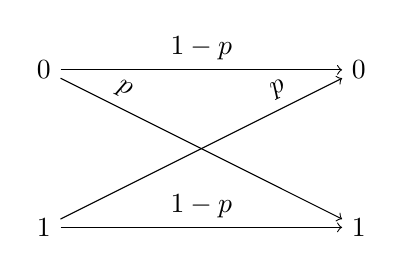
\begin{tikzpicture}
            \node[] (A) at (-2,0){$0$};
            \node[] (B) at (-2,-2){$1$};
            \node[] (A1) at (2,0){$0$};
            \node[] (B1) at (2,-2){$1$};
            \draw[->] (A) -- (A1)  node[midway, above]{$1-p$};
            \draw[->] (B) -- (B1) node[midway, above]{$1-p$};
            \draw[->] (A) -- (B1)  node[near start,sloped, above left]{$p$};
            \draw[->] (B) -- (A1) node[sloped,near end, above right]{$p$};
        \end{tikzpicture}

    \end{center}
    E poi la rappresentazione matriciale

    \begin{center}
        \begin{tikzpicture}
            \matrix (m)[matrix of math nodes,left delimiter=[,right delimiter={]},ampersand replacement=\&] {
                1-p  \& p \\
                p  \& 1-p \\
            };
            \node[] at (-1.9,0.3) {$0$};
            \node[] at (-1.9,-0.3) {$1$};
            \node[] at (-0.6,0.95) {$0$};
            \node[] at (0.60,0.95) {$1$};
            \node[] at (-1.9,0.95) {$X\backslash Y$};
        \end{tikzpicture}
    \end{center}

    \section{Capacità del canale}

    \begin{defi}
        La \textbf{capacità} del canale indica quanta informazione possiamo mandare sul canale.
    \end{defi}
    Formalmente è definita come

    $$C = \max_{p(x)} I(x,y)$$
    dove con $\max_{p(x)}$ prendiamo in considerazione tutte le possibili distribuzioni did $p(x)$, ovvero di probabilità di generare i simboli sorgenti. Calcoliamo le capacità per i canali precedenti:

    \begin{itemize}
        \item Canale binario senza rumore. Riscriviamo la capacità esprimendo l'informazione mutua
        $$C = \max_{p(X)} (H(X) - H(X|Y))$$
        Siccome dato $Y$ non abbiamo incertezza su $X$, allora $H(X|Y) = 0$, quindi
        $$= \max_{p(x)} H(X)$$
        Scegliendo $p(0) = \frac{1}{2}$ e $p(1) = \frac{1}{2}$ massimizziamo l'entropia che vale $1$ in questo caso. Allora la capacità del canale è proprio $1$.
        \item Canale binario simmetrico. Cominciamo con l'osservare che

        $$I(X,Y) = H(Y) - H(Y|X) = H(Y) - H(Y | X = 0) p(X = 0) - H(Y | X = 1) p(X = 1)$$
        Notiamo che

        $$H(Y|X = 0) = - p(y=0|x = 0)\log_2{p(y=0|x = 0)} -  p(y=1|x = 0)\log_2{p(y=1|x = 0)}$$
        $$= - (1-p) \log_2{(1-p)} - p\log_2{p} = H(p)$$
        Con $H(p)$ l'entropia di una bernoulliana di parametro $p$. Analogamente possiamo dimostrare che  $H(Y|X = 1) = H(p)$. Quindi la capacità del canale si riduce a

        $$C = \max_{p(x)} H(Y) - H(p)$$
        Non ci resta altro da fare che trovare il massimo valore di $H(Y)$. Cominciamo con analizzare $P(Y = 1)$

        $$P(Y = 1) = P(Y=1 | X = 0) P(X = 0) + P(Y=1 | X = 1) P(X = 1)$$
        $$= p P(X = 0) + (1-p) P(X = 1)$$
        Notiamo che  quando $P(X=1) = \frac{1}{2}$ abbiamo che $P(Y=1) = \frac{1}{2}$. Per questa scelta di $p(x)$ abbiamo che $H(Y) = 1$, ed è il massimo valore che può assumere. Possiamo quindi concludere che

        $$C =  1 - H(p)$$
    \end{itemize}



\end{document}